% This template has been downloaded from:
% http://www.latextemplates.com
%
% Original author:
% Ted Pavlic (http://www.tedpavlic.com)
%
% Modified by:
% Charles Newey (http://assemblyco.de)
%----------------------------------------

% Declare document
\documentclass{article}

% Packages
\usepackage{fancyhdr} % Required for custom headers
\usepackage{lastpage} % Required to determine the last page for the footer
\usepackage{extramarks} % Required for headers and footers
\usepackage{graphicx} % Images
\usepackage{tabularx} % Tables
\usepackage[table]{xcolor} % Table colours
\usepackage[colorlinks]{hyperref} % For URLs
\usepackage[T1]{fontenc} % Support symbols like < and >
\usepackage{lmodern} % Format symbols properly
\usepackage{listings} % Code highlighting

% Colours
\definecolor{negligible}{rgb}{0.55, 0.71, 0.0}
\definecolor{acute}{rgb}{1.0, 0.75, 0.0}
\definecolor{severe}{rgb}{1.0, 0.49, 0.0}
\definecolor{critical}{rgb}{0.9, 0.17, 0.31}

% Listings
\definecolor{javared}{rgb}{0.6,0,0} % for strings
\definecolor{javagreen}{rgb}{0.25,0.5,0.35} % comments
\definecolor{javapurple}{rgb}{0.5,0,0.35} % keywords
\definecolor{javadocblue}{rgb}{0.25,0.35,0.75} % javadoc

\lstset{language=Java,
	basicstyle=\ttfamily,
	keywordstyle=\color{javapurple}\bfseries,
	stringstyle=\color{javared},
	commentstyle=\color{javagreen},
	morecomment=[s][\color{javadocblue}]{/**}{*/},
	numbers=left,
	numberstyle=\tiny\color{black},
	stepnumber=2,
	numbersep=10pt,
	tabsize=4,
	showspaces=false,
	breaklines=true,
	showstringspaces=false}
	
\lstdefinelanguage{JavaScript}{
  keywords={typeof, new, true, false, catch, function, return, null, catch, switch, var, if, in, while, do, else, case, break},
  keywordstyle=\color{blue}\bfseries,
  ndkeywords={class, export, boolean, throw, implements, import, this},
  ndkeywordstyle=\color{darkgray}\bfseries,
  identifierstyle=\color{black},
  sensitive=false,
  comment=[l]{//},
  morecomment=[s]{/*}{*/},
  commentstyle=\color{purple}\ttfamily,
  stringstyle=\color{red}\ttfamily,
  morestring=[b]',
  morestring=[b]"
}

% Margins
\topmargin=-0.45in
\evensidemargin=0in
\oddsidemargin=0in
\textwidth=6.5in
\textheight=9.0in
\headsep=0.25in
\linespread{1} % Line spacing

% Other setup
\pagestyle{fancy}
\renewcommand\headrulewidth{0.4pt} % Size of the header rule
\renewcommand\footrulewidth{0.4pt} % Size of the footer rule
\setlength\parindent{0pt} % Removes all indentation from paragraphs
\renewcommand{\refname}{} % Removes bibliography title

% Set up constants
\newcommand{\address}{
\small{
	\begin{tabular}{ l}
		Department of Computer Science, \\
		Llandinam Building, \\
		Aberystwyth University, \\
		Aberystwyth, \\
		Ceredigion, \\
		SY23 3DB \\
	\end{tabular}
	}
}

% Set up the header and footer
\lhead{\doctitle}										% Top left header
\chead{\version}											% Top center head
\rhead{\firstxmark \status}								% Top right header
\lfoot{\lastxmark \qanumber}								% Bottom left footer
\cfoot{Aberystwyth University/Computer Science}			% Bottom center footer
\rfoot{Page\ \thepage\ of\ \protect\pageref{LastPage}}	% Bottom right footer

% Set up title page
\title{
	\vspace{1.2in}
	\textmd{\textbf{\doctitle}} \\
	\vspace{0.1in}\large{\textit{\today}} \\
	\vspace{0.4in}
	{\bf{\qanumber}} \\ \vspace{0.4in}
	\version \\
	\status \\
	\vspace{0.4in}
}

\author{\authors}
\date{}


%----------------------------- UPDATE THESE FOR EACH DOCUMENT ------------------------------
\newcommand{\version}{Version: 1.0} %======================================================= DOC VERSION
\newcommand{\status}{Status: Release} %===================================================== DOC STATUS
\newcommand{\qanumber}{SE.10.D3} %========================================================== QA NUMBER
\newcommand{\doctitle}{Group 10 Design Specification} %===================================== DOC TITLE

%----------------------------- UPDATE THESE FOR EACH DOCUMENT ------------------------------
%=========================================================================================== VERSION HISTORY
\newcommand{\versionhistory}{
		\begin{tabularx}{\linewidth}{| p{2cm} | p{2cm} | p{2cm} | X | }
			\hline
			\bf{Author} & \bf{Date} & \bf{Version} & \bf{Change made} \\
			\hline
			CCN & 03/12/2013 & 1.0 & Initial build of document \\
			\hline
			DEC & 04/12/2013 & 1.1 & Updated Markdown conversion issues \\
			\hline
			CCN & 04/12/2013 & 1.2 & Corrected spelling and grammar mistakes \\
			\hline
		\end{tabularx}
}

%=========================================================================================== AUTHOR LIST
\newcommand{\authors}{
	\begin{tabular}{| l | l |}
		\hline
		\bf{Contributor Name} & \bf{Role} \\
		\hline
		Daniel Clark & Project Lead \\
		\hline
		Mark Lewis & QA Manager \\
		\hline
		Charles Newey & Deputy Project Lead \& Android Developer \\
		\hline
		Martin Ferris & Android Developer \\
		\hline
		Ashley Iles & Android Developer \\
		\hline
		Kenny Packer & Android Developer \\
		\hline
		Stephen McFarlane & Deputy QA \& Web Developer \\
		\hline
		Kieran Palmer & Web Developer \\
		\hline
	\end{tabular}
	% Don't edit this
	\\ \\ \\ \\ \\ \\
	\address \vline
	\hspace{0.15in} \copyright Copyright Group 10, 2013
	% Don't edit this
}

% Make title page, ToC and other introductory elements
\begin{document}
	\maketitle
	\newpage
	\tableofcontents
	\newpage

	% Begin the actual document
	%================================================================================ DOCUMENT STARTS HERE
	\begin{section}{INTRODUCTION}
		\begin{subsection}{Purpose of This Document}
			The purpose of this document is to show that we have met the outlined objectives specified by the client.
		\end{subsection}
	
		\begin{subsection}{Scope}
			Scope
		\end{subsection}
		
		\begin{subsection}{Objectives}
			\begin{itemize}
				\item{Objective 1}
				\item{Objective 2}
			\end{itemize}
		\end{subsection}
	\end{section}
	
	
	
	\begin{section}{DECOMPOSITION DESCRIPTION}
		\begin{subsection}{Programs in System}
		The System that will be created will contain three systems; the Android app, a server and a web page. \\

		The Android side of the system will be used as the platform for the walking tour creator app. Within this app users can create a new tour, they will then be able to add locations to the tour. These locations will contain information such as the tours title, description, the way points of the location and possibly an image. Once the tour is saved and finished it can then be sent via Wi-Fi or internet connection on the device to the server. The data will be sent to the server as a Multimedia Internet Message Extension (MIME) format in an HTTP POST request.\\

		The server will be used to store all data about tours created on the Android app. On the server a database will be created and within the database a table for storing the tour's details. Once data is received a new record will be created and the data stored for easy re-use on the web page. To access this data the web page will use a PHP script with MySQL commands.\\

		The final program in the system is the web page, which will be used for displaying tours. On the website there will be a list of saved tours from which the user can click to view them. The tour will then be displayed on a map which will incorporate the use of the Google Maps API. By clicking on a Waypoint the user will be able to view the information added by the creator.
		\end{subsection}


	    \clearpage
	    \begin{subsection}{Significant Classes - Android}
		    \begin{subsubsection}{StumblrData}
		    This will be an abstract class which will contain variables and validation methods that other classes will use, such as "short description" and "title".
		    \end{subsubsection}

		    \begin{subsubsection}{Waypoint}
		    This class will handle all information and methods regarding locations on the route. A method will be used to create a Waypoint containing "title", "short description" and an image. Coordinates will be stored in a linked list of coordinates.
		    \end{subsubsection}

		    \begin{subsubsection}{Route}
		    This class will contain all the methods to handle all parts of creating a route, such as adding Waypoints to a linked list of Waypoints.
		    \end{subsubsection}
	    \end{subsection}
	
	    \begin{subsection}{Significant Classes - Web}
		    \subsubsection{Page}
		    The page class will make use of the Map and the Database Interaction classes. This class will be written in HTML and CSS, this class will display the map and web interface.

		    \subsubsection{Map}
		    The Map class will be the interface to the Google Maps API; which will be in JavaScript. This class will be used in conjunction with the database interaction to load information into the map in the web interface, along with other details which will be entered into the information box on each location. This class will be implemented using JavaScript and PHP.

		    \subsubsection{Database Interaction}
		    The database interaction class is where the database will be loaded; to be used to add and request data from the MySQL database. Included in the database will be the locations for the Maps API, as well as showing different tours in a table next to it markers for each route's Waypoints in another table. This class will implemented with PHP and MySQL.
	    \end{subsection}

    
    \begin{subsection}{Shared Modules Between Programs}
        As the two programs differ enormously in terms of the technology used, there are no common modules, per se. However, one could consider
    \end{subsection}


	\clearpage
	\begin{subsection}{Mapping Requirements to Classes}
        \begin{enumerate}
		    \item{FR1; Startup of software on Android device}
		    Android class Home and Android class AbstractActivity.

		    \item{FR2; Providing info about the whole walking tour}
		    Android class AbstractActivity, Android class DataEntryActivity
		    and Android class AbstractActivity.

		    \item{FR3; Adding locations to the walking tour}
		    Android class CreateWaypoint, Android class DataEntryActivity
		    and Android class AbstractActivity.

		    \item{FR4; Adding photos to the walks}
		    Android class CreateWaypoint, Android class DataEntryActivity 
		    and Android class AbstractActivity.

		    \item{FR5; Cancelling walks}
		    Android class CreateWaypoint and Android class AbstractActivity.

		    \item{FR6; Sending the walk to the server}
		    Android class FinishRoute and Android class AbstractActivity.

		    \item{FR7; Switching from the WTC}
		    Android class AbstractActivity.

		    \item{FR8; Trying out a created walking tour}
		    Web Page, Map and Database Interaction.

		    \item{FR9; Saving data on server}
		    Android class FinishRoute, Android class AbstractActivity, Web Page, Map and Database Interaction.
        \end{enumerate}
	\end{subsection}
\end{section}

\begin{section}{DEPENDENCY DESCRIPTION}
	\begin{subsection}{Class Diagrams - Inheritance Relationships}
		\begin{subsubsection}{Android Activity Classes}
			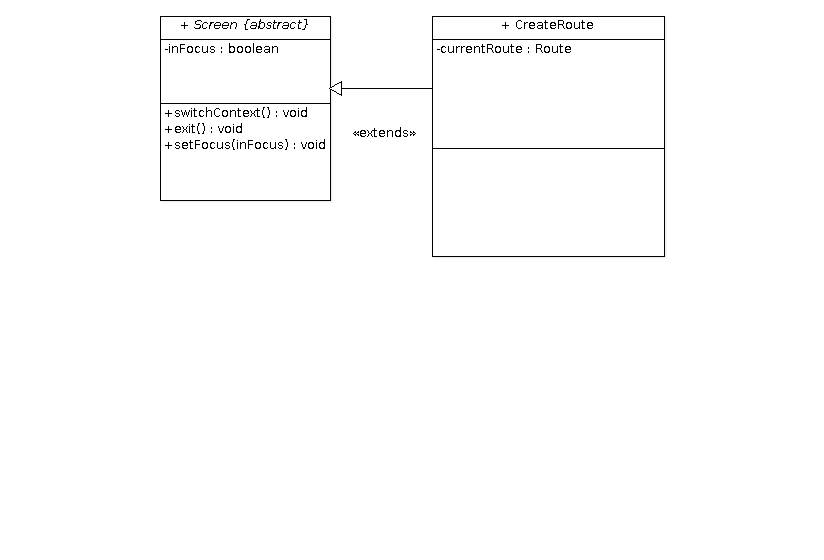
\includegraphics[angle=270,width=0.75\columnwidth]{../ClassDiagrams/InterfaceClassDiagram.png}
		\end{subsubsection}
		
		\clearpage
		\begin{subsubsection}{Android Data Classes}
			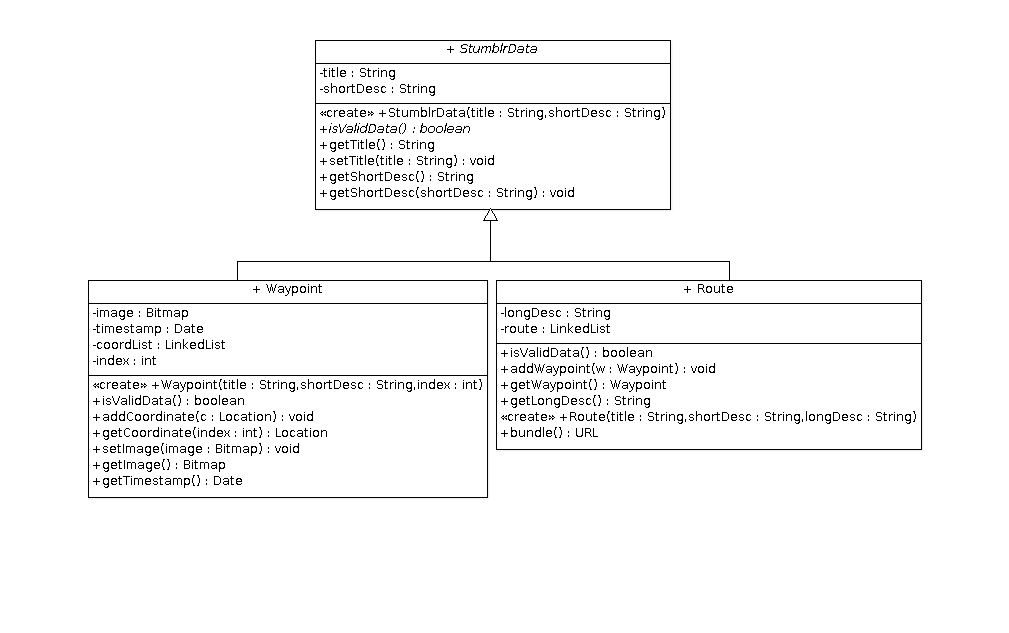
\includegraphics[angle=270,width=0.8\columnwidth]{../ClassDiagrams/DataStructuresClassDiagram.png}
		\end{subsubsection}
	\end{subsection}
\end{section}	
	
\begin{section}{DETAILED DESIGN}
	\clearpage
	\begin{subsection}{Significant Algorithms}
		\begin{subsubsection}{Upload Data}
		    \begin{enumerate}
		        \item{Bundle data}
		        \item{Cache Bundle}
		        \item{Send Bundle To Server}
		        \item{Display Progress bar in android drop down menu}
		        \item{Wait for confirmation...}
		        \item{If confirmation timeout reached... resend bundle.}
		    \end{enumerate}
		\end{subsubsection}
		
        \begin{subsubsection}{Bundle Data}
            \begin{enumerate}
                \item{Base 64 encode all images}
                \item{Collate data for each waypoint into JSON}
                \item{Collate every waypoint route metadata into JSON}
            \end{enumerate}
        \end{subsubsection}

        \begin{subsubsection}{Validate Inputs}
            \begin{enumerate}
                \item{Check if empty}
                \item{Check if contains "unsanitised" characters}
                \item{Check image sizes}
            \end{enumerate}
        \end{subsubsection}

        \begin{subsubsection}{Change Screen}
            \begin{enumerate}
                \item{Validate Inputs}
                \item{Display next screen}
            \end{enumerate}
        \end{subsubsection}
	\end{subsection}
\end{section}

\begin{section}{INTERFACE DESCRIPTION}
	\clearpage
	\begin{subsection}{Android Activities}
		\begin{subsubsection}{AbstractActivity \{abstract\}}
			\lstinputlisting[label=AbstractActivity,
			caption=AbstractActivity \{Abstract\}]{interfaces/AbstractActivity.java}
		\end{subsubsection}
	
		\clearpage
		\begin{subsubsection}{DataEntryActivity \{abstract\}}
			\lstinputlisting[label=DataEntryActivity,
			caption=DataEntryActivity \{Abstract\}]{interfaces/DataEntryActivity.java}
		\end{subsubsection}

		\begin{subsubsection}{Home}
			\lstinputlisting[label=Home,
			caption=Home]{interfaces/Home.java}
		\end{subsubsection}

		\clearpage
		\begin{subsubsection}{CreateRoute}
			\lstinputlisting[label=CreateRoute,
			caption=CreateRoute]{interfaces/CreateRoute.java}
		\end{subsubsection}

		\clearpage
		\begin{subsubsection}{CreateWaypoint}
			\lstinputlisting[label=CreateWaypoint,
			caption=CreateWaypoint]{interfaces/CreateWaypoint.java}
		\end{subsubsection}

		\clearpage
		\begin{subsubsection}{WaypointList}
			\lstinputlisting[label=WaypointList,
			caption=WaypointList]{interfaces/WaypointList.java}
		\end{subsubsection}

		\clearpage
		\begin{subsubsection}{FinishRoute}
			\lstinputlisting[label=FinishRoute,
			caption=FinishRoute]{interfaces/FinishRoute.java}
		\end{subsubsection}
	\end{subsection}

	\clearpage
	\begin{subsection}{Data Classes}
		\begin{subsubsection}{StumblrData \{abstract\}}
			\lstinputlisting[label=StumblrData,
			caption=StumblrData]{interfaces/data/StumblrData.java}
		\end{subsubsection}
		
		\clearpage
		\begin{subsubsection}{Route}
			\lstinputlisting[label=Route,
			caption=Route]{interfaces/data/Route.java}
		\end{subsubsection}
		
		\clearpage
		\begin{subsubsection}{Waypoint}
			\lstinputlisting[label=Waypoint,
			caption=Waypoint]{interfaces/data/Waypoint.java}
		\end{subsubsection}
	\end{subsection}
\end{section}

\clearpage
\begin{section}{DETAILED DESIGN}
	\begin{subsection}{Sequence Diagram}
		\begin{center}
			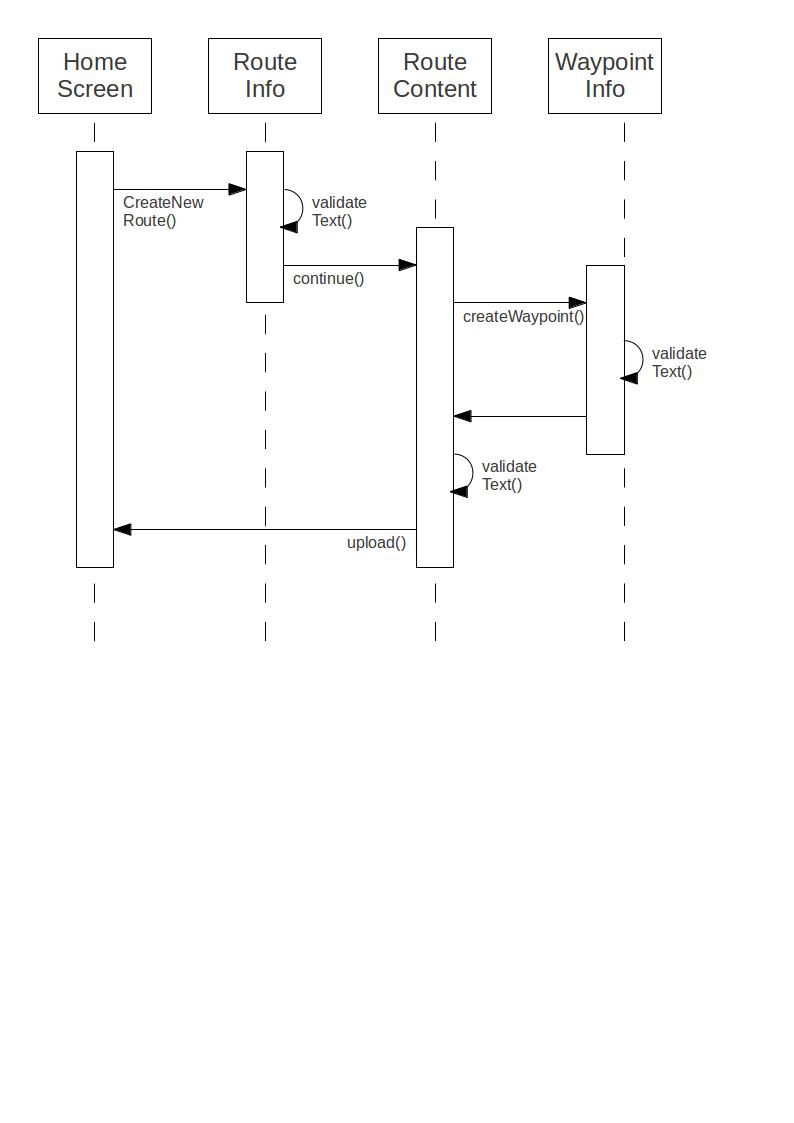
\includegraphics[width=0.9\columnwidth]{../SequenceDiagram/DetailedDesign5-1.jpg}
		\end{center}
	\end{subsection}
	
	\begin{subsection}{Significant Algorithms}
		\begin{subsubsection}{Upload Data}
		    \begin{enumerate}
		        \item{Bundle data}
		        \item{Cache Bundle}
		        \item{Send Bundle To Server}
		        \item{Display Progress bar in android drop down menu}
		        \item{Wait for confirmation...}
		        \item{If confirmation timeout reached... resend bundle.}
		    \end{enumerate}
		\end{subsubsection}
		
    \begin{subsubsection}{Bundle Data}
        \begin{enumerate}
            \item{Base 64 encode all images}
            \item{Collate data for each waypoint into JSON}
            \item{Collate every waypoint route metadata into JSON}
        \end{enumerate}
    \end{subsubsection}

    \begin{subsubsection}{Validate Inputs}
        \begin{enumerate}
            \item{Check if empty}
            \item{Check if contains "unsanitised" characters}
            \item{Check image sizes}
        \end{enumerate}
    \end{subsubsection}

    	\begin{subsubsection}{Change Screen}
    	    \begin{enumerate}
    	        \item{Validate Inputs}
    	        \item{Display next screen}
    	    \end{enumerate}
   		\end{subsubsection}
	\end{subsection}
	
	\begin{subsection}{Significant Data Structures - Android}
		The main classes in our design are the Route class, and the Waypoint class. 

		\begin{subsubsection}{Route}
			The route class is responsible for storing and processing all the information for one particular route. It does this by storing basic route information, plus a linked list of waypoints. We chose a linked list, as it's size is not fixed, meaning that we are not limited in terms of how many waypoints we can have. We chose a linked list over an arraylist, as an arraylist would be innefficeint and slow, due to the processes involved when adding new items.
		\end{subsubsection}

		\begin{subsubsection}{Waypoint}
			The waypoint class is responsible for storing and processing the data for each waypoint along the route. It does this by storing basic route information, plus a linked list of co-ordinates between the current waypoint and the previous waypoint. The timestamp is also generated when the waypoint is constructed. It can also store an optional image, if the user so wishes to add one.
		\end{subsubsection}

		\begin{subsubsection}{Co-ordinates}
			The android.location.Location class from the Android API will be used for storing Coordinates.
		\end{subsubsection}
	\end{subsection}

	\begin{subsection}{Significant Data Structures - MySQL Database}
	To store data about tours a database will be used, this will use MySQL and be the gateway between the android program and the web program. The database shall contain the four tables below with the relevent columns.

		\begin{subsubsection}{List of Walks}
			Each walk is listed in the "walks" table. There is one record for each walk, and the record has 
		the following characteristics. An ID which is used to order the list of the walks, it will be the primary key for the record and generated by the database. Each walk has a title which represents the name of the walk set by the user and will be of type varchar. The tour also has both short and long descriptions. The short description is a short summary of the walk, where as the long description goes into more detail about the tour. Both of these columns will be varchars. The tour also contains details of how long the walk will take and this will be stored as a float in the database. This will be generated by taking a time for the start of the walk and a time when the walk is finished, then calculating the difference. The final data stored about a walk is the distance and this will also be stored as a float. To create this value the distance between each waypoint will be added.
		\end{subsubsection}
		
		\begin{subsubsection}{Location}
			In this table basic details will be stored about each Waypoint within the walk. The primary key in is the ID and will be generated by the database. This table also uses a foreign key to reference which walk is part of in the walks table, which will be called walkID. Next in the table are two columns for longitude and latitude, both of which are stored as floats. Finally the last column in the table is the timestamp and this will be stored as a float.
		\end{subsubsection}

		\begin{subsubsection}{Place Description}
			This table is used to store extra details about each waypoint within a walk. Therefore this table needs an ID as primary key and also a foreign key to link to the location table, which will be called locationID. There is also a column for description which gives a description about the Waypoint. The description will be of type varchar.
\end{subsubsection}
		
		\begin{subsubsection}{Photo Usage}
			This table is very similar to the place description table, but stores a file path to an image of the location. The table needs to have a primary key (id) for each image as well as a foreign key linked to the location which it is about (placeID). The final column in the table is a varchar which stores the Base64 representation of an image - "photoData".
		\end{subsubsection}

		\clearpage
		\begin{subsubsection}{JSON}
			\begin{lstlisting}
{
	"Walk": {
		"walkTitle": "Road Rummer",
		"shortDescription": "meep meep!",
		"longDescription": "meep meep meep meep!",
		"walkHours": 42,
		"walkDistance": 42,
		"Locations": [
			{
				"LocationTitle",
				"GPSTraces" : [
					{
						"latitude": 42.00000,
						"longitude": 42.00000
					}
				],
				"timestamp": 16:20,
				"locationDescription": "This is a bar, can you say bar?",
				"Photo": {
					"photoName": "Photo of Rummers",	
					"64bitPhoto": gfkfhjfhkhfctyb7r67tny8b6n756
				}
			}
		]
	}
}
			\end{lstlisting}
		\end{subsubsection}
	\end{subsection}
	
	\begin{subsection}{Website Interface Specification}
		The web interface will use all of these classes to create a page that will load in a database of routes that the user will be able to view a route map from. The user will also be able to choose from a range of tours provided right next to the map. 

		\subsubsection{Page}
			The page class is the web page that will hold the map and database interaction. This class will be the way the interface is shown by using css. This class will hold the map class and the database interaction class. The page class will be done in HTML and it will validate to XHTML 1.0 Strict. 

		\subsubsection{Map}
			The map class is the class which holds the Google maps API which will be in JavaScript. This class holds functions that are provided from the google maps API website that initialise the maps and the pointers on the map. There also other function such as myclick() which records when the user click on the map. Also there is a createMarker() function which will create an info box for each point provided this is were we will provide the information for each place by using the database interaction here to create all the pointers.
		>Here are the functions and javacript I will using from the Google Maps API website that will be working with the database interaction.

		\subsubsection{Database Interaction}
			The database interaction class is where the web page will connect to the databases then It will use jquery to get all the points on the tour that the user choose. It will present the tours as links to the left of the map which when clicked will connect to that database and load in all the points to the map and load pointer to the right of the map. The map will have information boxes for each point on the map which have had information put in them by using Jquery as the information for each point is save alongside the coordinates. A thumbnail of an image of the location will also be in these information boxes and when clicked on a bigger image will show at the centre of the page. PHP code will be used to read in the databases of tours which will contain each tours the code will create links on the left of the map to bring up a new tour and load in the poiner. The PHP code used  will mostly be in the create pointer part of the map class where it will create pointer for each entry in the database which will then create a link on the right of the map to link to each pointer on the map.

		\subsubsection{Google Maps API JavaScript Example}
		\begin{lstlisting}[caption=Google Maps API Javascript Example]
<script type="text/javascript"> 
  var side_bar_html = ""; 
  var gmarkers = []; 
  var map = null;
  
  
//initializes the Google Map.
function initialize() {
// create the map
	var myOptions = {
		zoom: 15,
		//sets the map to Aberytwyth
		center: new google.maps.LatLng(52.4140,-4.0810),
		mapTypeControl: true,
		mapTypeControlOptions: {style: google.maps.MapTypeControlStyle.DROPDOWN_MENU},
		navigationControl: true,
		mapTypeId: google.maps.MapTypeId.ROADMAP
	}
	
map = new google.maps.Map(document.getElementById("map_canvas"), myOptions);

	google.maps.event.addListener(map, 'click', function() {
		infowindow.close();
	});

	//creates pointers - this will be used with the database interaction class
	var point = new google.maps.LatLng(,);
	var marker = createMarker(point,"NAME","DESCRIPTION")

	document.getElementById("side_bar").innerHTML = side_bar_html;
}

//creates the map and set the size of the map.
var infowindow = new google.maps.InfoWindow(
{ 
  size: new google.maps.Size(200,75)
});
  

function myclick(i) {
	google.maps.event.trigger(gmarkers[i], "click");
}

function createMarker(latlng, name, html) {
  var contentString = html;
  var marker = new google.maps.Marker({
      position: latlng,
      map: map,
      zIndex: Math.round(latlng.lat()*-100000)<<5
      });

  google.maps.event.addListener(marker, 'click', function() {
      infowindow.setContent(contentString); 
      infowindow.open(map,marker);
      });
  
  gmarkers.push(marker);
  side_bar_html += '<a href="javascript:myclick(' + (gmarkers.length-1) + ')">' + name + '<\/a><br>';
}
</script>
		\end{lstlisting}
	\end{subsection}
\end{section}
	
\begin{section}{Android Design Justifications}
	\begin{itemize}
		\item{We decided to implement Base64 encoding on our images within our application - this allows the developers to directly embed the Base64-encoded image data within the webpage - and it's a simple API call to convert to Base64 within Android.}
		\item{We also decided to use JSON within the MIME/HTTP POST request. This would allow us to transfer data between client and server in a much more human-readable (and therefore maintainable) manner. Furthermore, JSON is a much more modern standard than mimicking an HTTP form POST, and just as simple to implement. The team spoke to the customer, and they approved the design change.}
	\end{itemize}
\end{section}

\begin{section}{Web Design Justifications}
	\begin{itemize}
		\item{We decided to use the Aberystwyth Users web server (\href{users.aber.ac.uk}{http://users.aber.ac.uk/}) for hosting the website. This is because it is fast, reliable, well-maintained and stable, as well as running on a solid Linux platform. The server also runs our chosen services - namely PHP and MySQL. We chose those two technologies as PHP is a long-recognised and popular web programming language, and MySQL has an enormous user base and is extremely stable, as well as implementing all of the SQL statements we plan to use.}
		\item{Google Maps was chosen for its simple and well-documented API, as well it's flexible JavaScript library. It also has a very well-known and highly attractive interface, which fits in with our interface design plan.}
	\end{itemize}
\end{section}

% Include references here (edit the References.bib file)
\nocite{LaTeXTemplate} % DO NOT EDIT
\nocite{LaTeXListings}
\nocite{LaTeXListings2}
\nocite{LaTeXListings3}
\nocite{JavaScriptReference}
\nocite{AndroidReference}

% Format bibliography/refs
\newpage
\begin{section}{REFERENCES}
	\bibliographystyle{acm}
	\bibliography{References}
\end{section}

\vspace{1cm}
\begin{section}{VERSION HISTORY}
	\versionhistory
\end{section}
\end{document}

%									Useful bits and pieces
%\begin{section}{section_name}									% Start section
%\end{section}													% End section
%\begin{center} \end{center}									% Center stuff
%\includegraphics[width=0.75\columnwidth]{example_figure}		% Insert image
%\clearpage														% Clear page after section
%\url{http://www.google.com/} 									% Include URL
%\nocite{citationName}											% Cite to bibliography (but not to text)
%\cite{citationName}											% Include reference